\documentclass[11pt,a4paper]{article}

\usepackage[french]{babel}
\usepackage{geometry}
\geometry{margin=2.2cm}
\usepackage{graphicx}
\usepackage{xcolor}
\usepackage{booktabs}
\usepackage{array}
\usepackage{listings}
\usepackage{caption}
\usepackage{titlesec}
\usepackage{fancyhdr}
\usepackage{hyperref}
\usepackage{enumitem}

\definecolor{codebg}{RGB}{245,246,248}
\definecolor{codeframe}{RGB}{205,210,218}
\definecolor{linkblue}{RGB}{16,78,139}
\definecolor{okgreen}{RGB}{22,120,60}
\definecolor{failred}{RGB}{170,30,30}

\hypersetup{colorlinks=true, linkcolor=linkblue, urlcolor=linkblue, citecolor=linkblue}

\lstdefinestyle{shell}{
  backgroundcolor=\color{codebg},
  frame=single,
  rulecolor=\color{codeframe},
  basicstyle=\ttfamily\scriptsize,
  breaklines=true,
  breakatwhitespace=false,
  columns=fullflexible,
  keepspaces=true,
  showstringspaces=false,
  literate={é}{{\'e}}1 {è}{{\`e}}1 {à}{{\`a}}1 {ç}{{\c c}}1 {û}{{\^u}}1 {ô}{{\^o}}1,
  captionpos=b
}
\lstset{style=shell}

\titleformat{\section}{\large\bfseries\color{linkblue}}{\thesection.}{0.6em}{}
\titleformat{\subsection}{\normalsize\bfseries}{\thesubsection}{0.5em}{}

\pagestyle{fancy}
\fancyhf{}
\fancyhead[L]{\footnotesize DevOps \& Cloud Computing --- Lab No. 07}
\fancyhead[R]{\footnotesize Sadoune Fadjr --- Groupe 02 --- ING 5}
\fancyfoot[C]{\footnotesize\thepage}
\renewcommand{\headrulewidth}{0.4pt}

\newcommand{\success}{\textcolor{okgreen}{\textbf{SUCCESS}}}
\newcommand{\failure}{\textcolor{failred}{\textbf{FAILURE}}}

\begin{document}

\begin{titlepage}
\centering
\vspace*{1.2cm}
{\large Département d'Informatique}\\[0.3cm]
{\large 5\textsuperscript{e} année --- Ingénierie Logicielle (ING 5)}\\[2.0cm]

{\Huge\bfseries Rapport de TP No. 07}\\[0.6cm]
{\LARGE Building a CI/CD Pipeline\\[0.2cm] with Jenkins and Docker}\\[2.2cm]

\rule{\linewidth}{0.4pt}\\[0.6cm]
{\large\bfseries Réalisé par}\\[0.3cm]
{\Large Sadoune Fadjr}\\[0.3cm]
{\large Groupe 02 --- ING 5}\\[0.6cm]
\rule{\linewidth}{0.4pt}\\[2.0cm]

{\large Module : DevOps \& Cloud Computing}\\[3.0cm]

{\large Année universitaire 2026--2027}\\[0.3cm]
{\large \today}
\vfill
\end{titlepage}

\tableofcontents
\newpage

\section{Introduction et objectifs}

Ce rapport présente la réalisation du TP No. 07 : la construction d'un pipeline
d'intégration et de livraison continues (CI/CD) avec \textbf{Jenkins} et \textbf{Docker}
autour d'une petite application \textbf{Flask}.

Les objectifs du TP sont les suivants :
\begin{itemize}[leftmargin=1.2cm]
  \item expliquer le rôle de Jenkins dans l'intégration continue et la livraison continue ;
  \item comprendre les composants principaux d'un pipeline Jenkins ;
  \item connecter un job Jenkins à un dépôt GitHub ;
  \item construire automatiquement une image Docker ;
  \item exécuter des tests automatisés dans le pipeline ;
  \item déployer l'application et vérifier qu'elle est disponible ;
  \item constater qu'un test en échec empêche le déploiement d'une version défectueuse.
\end{itemize}

Le travail a été réalisé sur un poste \textbf{Windows} avec \textbf{Docker Desktop}
(conteneurs Linux), Jenkins étant lui-même exécuté dans un conteneur Docker.
Deux adaptations ont été nécessaires par rapport à l'énoncé prévu pour une machine Linux :
\begin{enumerate}[leftmargin=1.2cm]
  \item l'image Jenkins officielle ne contient pas le client Docker, il a donc fallu
        construire une image dérivée contenant le binaire \texttt{docker} et monter le
        socket Docker sur le conteneur Jenkins ;
  \item les étapes \texttt{curl} de vérification utilisent le nom du conteneur
        applicatif (réseau Docker partagé) et \texttt{host.docker.internal} au lieu de
        \texttt{localhost}, car \texttt{localhost} désigne le conteneur Jenkins lui-même.
\end{enumerate}

\section{Architecture et environnement}

\subsection{Architecture du flux}

Le flux du TP est le suivant :
\begin{center}
\textbf{GitHub} $\rightarrow$ \textbf{Jenkins Pipeline} $\rightarrow$
\textbf{Docker Image} $\rightarrow$ \textbf{Docker Container} $\rightarrow$
\textbf{Flask Application}
\end{center}

L'application est exposée sur \texttt{http://localhost:8081} et Jenkins sur
\texttt{http://localhost:8080}.

\subsection{Environnement technique}

\begin{table}[h!]
\centering
\caption{Versions utilisées sur le poste de travail}
\begin{tabular}{@{}ll@{}}
\toprule
Composant & Version / configuration \\
\midrule
Système & Windows, Docker Desktop 4.50.0 (conteneurs Linux) \\
Moteur Docker & 28.5.1 \\
Client Docker (dans le conteneur Jenkins) & 28.5.1 (binaire statique) \\
Jenkins & 2.541.3 (image \texttt{jenkins/jenkins:lts-jdk17}) \\
Image Jenkins personnalisée & \texttt{jenkins-docker-lab} \\
Git & 2.47.3 \\
Python de l'application & 3.12 (\texttt{python:3.12-slim}) \\
pytest & 9.2.0 \\
\bottomrule
\end{tabular}
\end{table}

\subsection{Conteneurisation de Jenkins}

L'image \texttt{jenkins-docker-lab} est construite à partir de
\texttt{jenkins/jenkins:lts-jdk17} et ajoute le client Docker ainsi que
\texttt{curl} :

\begin{lstlisting}[caption={Dockerfile de l'image Jenkins (hors dépôt applicatif).}]
FROM jenkins/jenkins:lts-jdk17
USER root
RUN apt-get update \
    && apt-get install -y --no-install-recommends ca-certificates curl \
    && rm -rf /var/lib/apt/lists/* \
    && curl -fsSL https://download.docker.com/linux/static/stable/x86_64/docker-28.5.1.tgz \
       | tar xz -C /tmp \
    && mv /tmp/docker/docker /usr/local/bin/docker \
    && rm -rf /tmp/docker
USER jenkins
\end{lstlisting}

Le conteneur Jenkins est lancé avec le socket Docker monté et sur un réseau dédié
partagé avec le conteneur applicatif :

\begin{lstlisting}
docker network create jenkins-net
docker run -d --name jenkins --network jenkins-net -u root \
  -p 8080:8080 -p 50000:50000 \
  -v //var/run/docker.sock:/var/run/docker.sock \
  -v jenkins_home:/var/jenkins_home jenkins-docker-lab
\end{lstlisting}

\section{Structure du projet et dépôt GitHub}

\subsection{Structure du dépôt}

\begin{lstlisting}
jenkins-flask-lab/
|-- app.py
|-- requirements.txt
|-- Dockerfile
|-- Jenkinsfile
|-- tests/
|   `-- test_app.py
`-- (fichiers annexes : .gitignore, .gitattributes, RAPPORT_Lab07.md)
\end{lstlisting}

Le dépôt public est disponible à l'adresse :
\url{https://github.com/Sadoune321/jenkins-flask-lab}

\subsection{Application Flask}

\begin{lstlisting}[caption={app.py}]
import os
from flask import Flask, jsonify

app = Flask(__name__)

@app.route("/")
def home():
    version = os.getenv("APP_VERSION", "local")
    return f"<h1>Jenkins CI/CD Lab</h1><p>Version: {version}</p>"

@app.route("/health")
def health():
    return jsonify(status="ok"), 200

if __name__ == "__main__":
    app.run(host="0.0.0.0", port=8000)
\end{lstlisting}

\subsection{Dépendances et Dockerfile}

\begin{lstlisting}[caption={requirements.txt}]
Flask
pytest
gunicorn
\end{lstlisting}

\begin{lstlisting}[caption={Dockerfile de l'application.}]
FROM python:3.12-slim
WORKDIR /app
COPY requirements.txt .
RUN pip install --no-cache-dir -r requirements.txt
COPY app.py .
COPY tests ./tests
ENV PYTHONPATH=/app
EXPOSE 8000
CMD ["gunicorn", "--bind", "0.0.0.0:8000", "app:app"]
\end{lstlisting}

La ligne \texttt{ENV PYTHONPATH=/app} a été ajoutée après un premier échec du pipeline :
pytest ne trouvait pas le module \texttt{app} lors de l'import
(\texttt{ModuleNotFoundError: No module named 'app'}), car le répertoire de travail
n'était pas dans le chemin Python lors de l'exécution des tests dans le conteneur.

\subsection{Tests automatisés}

\begin{lstlisting}[caption={tests/test\_app.py}]
from app import app

def test_home():
    response = app.test_client().get("/")
    assert response.status_code == 200
    assert b"Jenkins CI/CD Lab" in response.data

def test_health():
    response = app.test_client().get("/health")
    assert response.status_code == 200
    assert response.get_json() == {"status": "ok"}
\end{lstlisting}

\section{Le pipeline Jenkins}

\subsection{Le Jenkinsfile}

Le pipeline déclaratif comporte cinq étapes : Checkout, Build, Test, Deploy et Verify.

\begin{lstlisting}[caption={Jenkinsfile (version Linux utilisée par Jenkins).}]
pipeline {
    agent any
    environment {
        IMAGE_NAME     = 'jenkins-flask-lab'
        CONTAINER_NAME = 'jenkins-flask-app'
        APP_PORT       = '8081'
        NETWORK_NAME   = 'jenkins-net'
    }
    stages {
        stage('Checkout') {
            steps { echo 'Source code is available in the workspace.' }
        }
        stage('Build') {
            steps { sh 'docker build -t ${IMAGE_NAME}:${BUILD_NUMBER} .' }
        }
        stage('Test') {
            steps { sh 'docker run --rm ${IMAGE_NAME}:${BUILD_NUMBER} pytest -v' }
        }
        stage('Deploy') {
            steps {
                sh '''
                    docker rm -f ${CONTAINER_NAME} || true
                    docker run -d --network ${NETWORK_NAME} --name ${CONTAINER_NAME} \
                        -p ${APP_PORT}:8000 -e APP_VERSION=${BUILD_NUMBER} \
                        ${IMAGE_NAME}:${BUILD_NUMBER}
                '''
            }
        }
        stage('Verify') {
            steps {
                sh 'curl --fail --retry 10 --retry-delay 2 http://${CONTAINER_NAME}:8000/health'
                sh 'curl --fail http://${CONTAINER_NAME}:8000/'
                sh 'curl --fail http://host.docker.internal:${APP_PORT}/health'
            }
        }
    }
    post {
        success { echo 'Pipeline completed successfully.' }
        failure { echo 'Pipeline failed. Check the stage that reported an error.' }
    }
}
\end{lstlisting}

\subsection{Description des étapes}

\begin{table}[h!]
\centering
\caption{Rôle de chaque étape du pipeline}
\begin{tabular}{@{}p{2.1cm}p{6.3cm}p{5.4cm}@{}}
\toprule
Étape & Action de Jenkins & Résultat attendu \\
\midrule
Checkout & Récupération du dépôt configuré dans le job (« Pipeline script from SCM ») & Code et Jenkinsfile disponibles dans le workspace \\
Build & \texttt{docker build -t jenkins-flask-lab:\${BUILD\_NUMBER} .} & Image taguée avec le numéro de build \\
Test & \texttt{docker run --rm ... pytest -v} & 2 tests passent, sinon arrêt du pipeline \\
Deploy & Suppression de l'ancien conteneur puis démarrage du nouveau & Nouvelle version démarrée sur le port 8081 \\
Verify & Requêtes HTTP sur \texttt{/health} et \texttt{/} avec réessais & L'application répond correctement \\
\bottomrule
\end{tabular}
\end{table}

\subsection{Configuration du job dans Jenkins}

Le job a été créé avec le nom \texttt{jenkins-flask-lab}, de type \textbf{Pipeline},
puis configuré en \emph{Pipeline script from SCM} avec :
\begin{itemize}[leftmargin=1.2cm]
  \item SCM : Git ;
  \item Repository URL : \url{https://github.com/Sadoune321/jenkins-flask-lab.git} (dépôt public, sans credentials) ;
  \item Branch Specifier : \texttt{*/main} ;
  \item Script Path : \texttt{Jenkinsfile}.
\end{itemize}

\begin{figure}[h!]
\centering
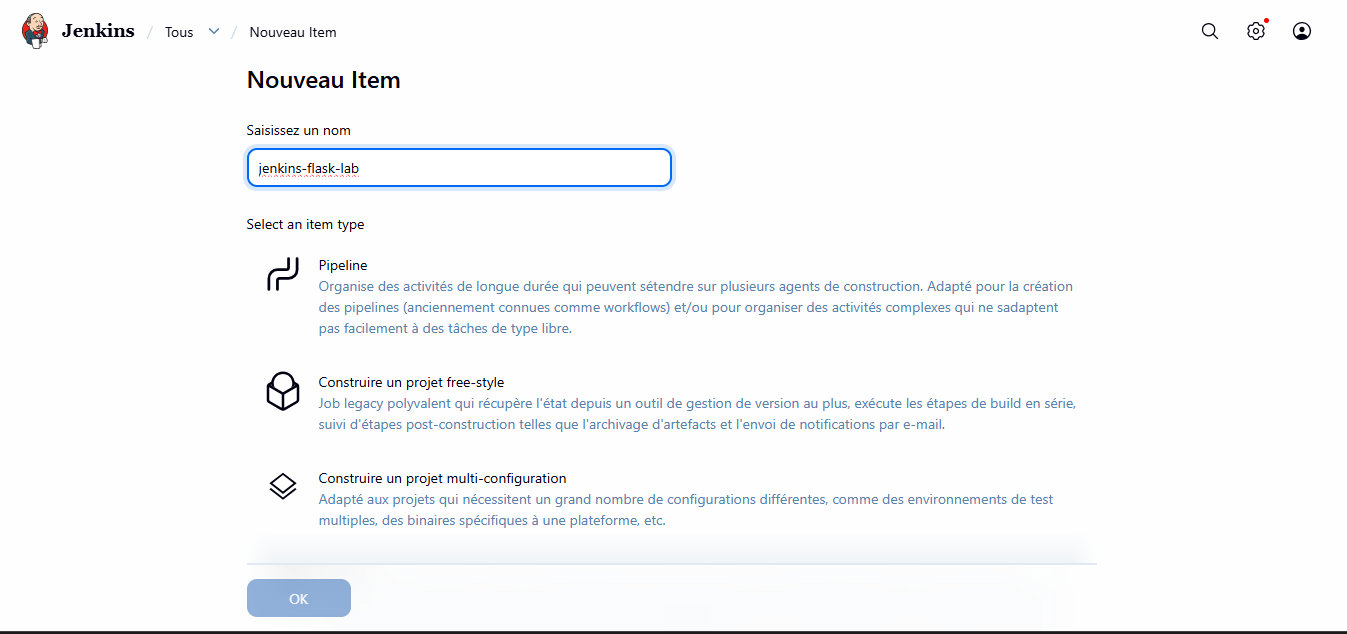
\includegraphics[width=0.92\textwidth]{img/jenkins_new_item.png}
\caption{Création du job Pipeline \texttt{jenkins-flask-lab} dans Jenkins.}
\end{figure}

\section{Résultats : pipeline réussi}

Le pipeline s'exécute avec succès : les cinq étapes sont vertes, l'image est construite
et taguée avec le numéro de build, les deux tests passent, le conteneur est déployé et
les vérifications HTTP réussissent.

\begin{figure}[h!]
\centering
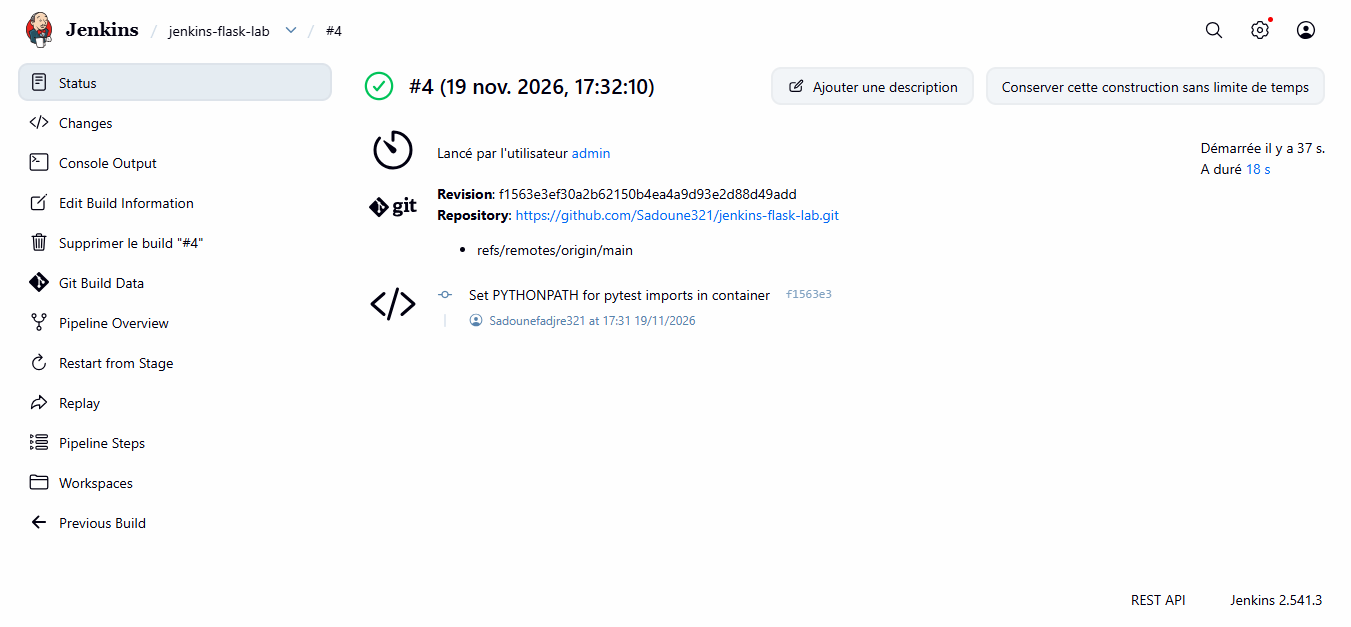
\includegraphics[width=0.92\textwidth]{img/build_success.png}
\caption{Build réussi : le pipeline se termine avec le statut SUCCESS.}
\end{figure}

\begin{figure}[h!]
\centering

\includegraphics[width=0.92\textwidth]{img/app_home.png}
\caption{Application déployée accessible sur \texttt{http://localhost:8081} : le numéro de build est affiché.}
\end{figure}

\begin{figure}[h!]
\centering
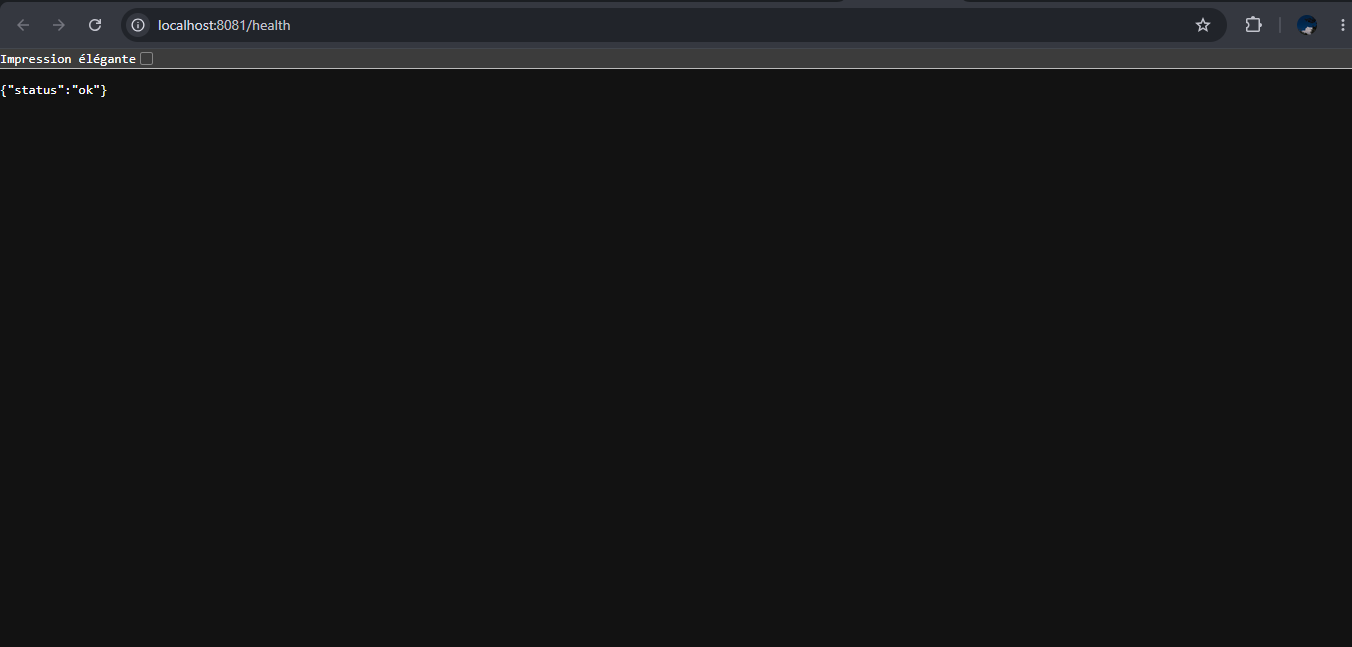
\includegraphics[width=0.92\textwidth]{img/app_health.png}
\caption{Point de contrôle \texttt{/health} : réponse \texttt{\{"status":"ok"\}}.}
\end{figure}

Sortie console condensée d'un build réussi (build 7) :

\begin{lstlisting}
Started by user admin
Checking out Revision fe1a225 (refs/remotes/origin/main)
[Checkout] Source code is available in the workspace.
[Build]    + docker build -t jenkins-flask-lab:7 .
           Successfully tagged jenkins-flask-lab:7
[Test]     + docker run --rm jenkins-flask-lab:7 pytest -v
           tests/test_app.py::test_home PASSED      [ 50%]
           tests/test_app.py::test_health PASSED    [100%]
           2 passed in 0.30s
[Deploy]   + docker rm -f jenkins-flask-app || true
           + docker run -d --network jenkins-net --name jenkins-flask-app
             -p 8081:8000 -e APP_VERSION=7 jenkins-flask-lab:7
[Verify]   + curl --fail --retry 10 --retry-delay 2 .../health
           {"status":"ok"}
           <h1>Jenkins CI/CD Lab</h1><p>Version: 7</p>
Pipeline completed successfully.
Finished: SUCCESS
\end{lstlisting}

\section{Partie E : observation d'un pipeline en échec}

Pour démontrer que les tests protègent la production, l'assertion du test de santé a été
temporairement modifiée :

\begin{lstlisting}
assert response.get_json() == {"status": "incorrect"}
\end{lstlisting}

Après commit et push (commit \texttt{dd81f24}, message
« Introduce a test failure »), un nouveau build (build 8) est lancé. Comme prévu :
\begin{itemize}[leftmargin=1.2cm]
  \item l'étape \textbf{Test} échoue ;
  \item les étapes \textbf{Deploy} et \textbf{Verify} sont ignorées (\emph{skipped}) ;
  \item le build se termine en \failure{} ;
  \item le conteneur de la version précédente reste en service et n'est pas remplacé.
\end{itemize}

\begin{figure}[h!]
\centering
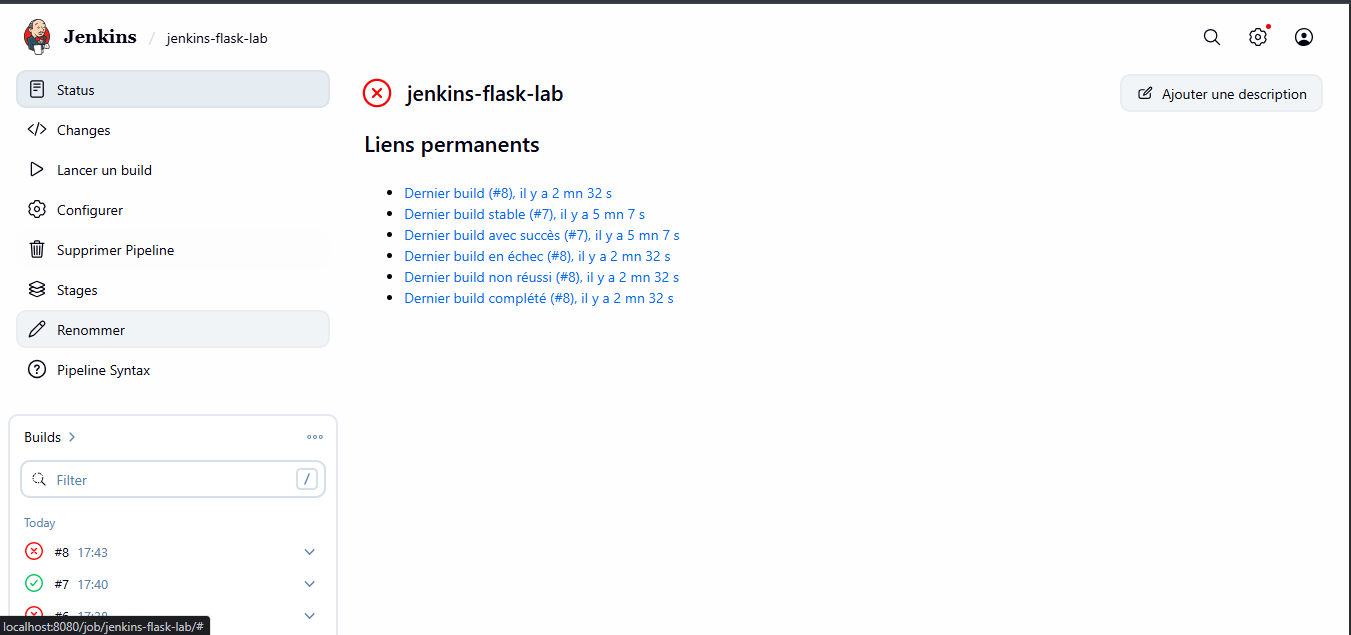
\includegraphics[width=0.92\textwidth]{img/build_failure.png}
\caption{Build 8 en échec après introduction volontaire d'un test défaillant.}
\end{figure}

\begin{lstlisting}[caption={Extrait de la console du build 8 (échec attendu).}]
+ docker build -t jenkins-flask-lab:8 .
Successfully tagged jenkins-flask-lab:8
tests/test_app.py::test_home PASSED                                      [ 50%]
tests/test_app.py::test_health FAILED                                    [100%]

    def test_health():
        response = app.test_client().get("/health")
        assert response.status_code == 200
>       assert response.get_json() == {"status": "incorrect"}
E       AssertionError: assert {'status': 'ok'} == {'status': 'incorrect'}

Stage "Deploy" skipped due to earlier failure(s)
Stage "Verify" skipped due to earlier failure(s)
Pipeline failed. Check the stage that reported an error.
ERROR: script returned exit code 1
Finished: FAILURE
\end{lstlisting}

\subsection{Explication}

La version défectueuse n'a pas été déployée car le pipeline est conçu pour s'arrêter dès
qu'une étape échoue : les étapes suivantes ne sont pas exécutées. Le conteneur
\texttt{jenkins-flask-app} continue donc de servir la dernière version valide. C'est
exactement le comportement attendu d'un pipeline CI/CD : \emph{on ne publie pas une
version dont les tests échouent}. L'assertion correcte a ensuite été rétablie
(commit \texttt{ed7a651}, « Fix health test ») et un nouveau build a été programmé.

\section{Diagnostics et sorties de commandes}

\subsection{Conteneurs actifs}

\begin{lstlisting}
$ docker ps
NAMES               IMAGE                 STATUS          PORTS
jenkins-flask-app   jenkins-flask-lab:7   Up 14 minutes   0.0.0.0:8081->8000/tcp
jenkins             jenkins-docker-lab    Up 27 minutes   0.0.0.0:8080->8080/tcp, 0.0.0.0:50000->50000/tcp
\end{lstlisting}

\subsection{Vérification du client et du serveur Docker depuis Jenkins}

\begin{lstlisting}
$ docker exec jenkins docker version --format "Client {{.Client.Version}} / Server {{.Server.Version}}"
Client 28.5.1 / Server 28.5.1
\end{lstlisting}

\subsection{Images applicatives construites par Jenkins}

\begin{lstlisting}
$ docker images jenkins-flask-lab
REPOSITORY           TAG   SIZE
jenkins-flask-lab    2     220MB
jenkins-flask-lab    3     220MB
jenkins-flask-lab    4     220MB
jenkins-flask-lab    5     220MB
jenkins-flask-lab    6     220MB
jenkins-flask-lab    7     220MB
jenkins-flask-lab    8     220MB
\end{lstlisting}

\subsection{Vérification fonctionnelle depuis le poste Windows}

\begin{lstlisting}
$ curl -s http://localhost:8081/health
{"status":"ok"}

$ curl -s http://localhost:8081/
<h1>Jenkins CI/CD Lab</h1><p>Version: 7</p>
\end{lstlisting}

\section{Partie F : Blue-Green deployment et rollback (questions 19)}

\subsection{Différence entre deployment et release}
Le \emph{deployment} est l'opération technique qui installe et démarre une nouvelle
version dans un environnement (par exemple Green). La \emph{release} est le moment où
cette version est réellement exposée aux utilisateurs (bascule du trafic). On peut donc
déployer sans publier : la nouvelle version tourne en Green mais aucun utilisateur n'y
accède avant la bascule. Le deployment est une décision technique, la release une
décision produit/métier.

\subsection{Pourquoi déployer la nouvelle version sur Green avant le trafic ?}
Parce que Green est un environnement identique à la production mais isolé du trafic réel.
On peut y valider la version (tests, health checks, monitoring) sans aucun risque pour les
utilisateurs, qui continuent d'utiliser Blue. Un défaut détecté n'a alors aucune
conséquence visible.

\subsection{Quel composant peut router les requêtes vers Blue ou Green ?}
Un \emph{reverse proxy} ou un répartiteur de charge : \textbf{NGINX} (cité dans le TP),
mais aussi HAProxy, un load balancer cloud ou le DNS. La bascule consiste à modifier
l'upstream puis à recharger la configuration du proxy.

\subsection{Pourquoi Blue doit-il rester disponible après la bascule ?}
Pour permettre un \emph{rollback} immédiat : si un problème apparaît sur Green, on
renvoie le trafic vers Blue qui exécute encore la version stable. Blue sert de filet de
sécurité pendant la période d'observation.

\subsection{Comment Jenkins peut-il automatiser déploiement, tests et approbation ?}
Un pipeline étendu peut : construire l'image, déployer le conteneur Green, exécuter les
tests et health checks sur Green, attendre une approbation manuelle (étape \texttt{input}
ou plugin d'approbation), puis modifier la configuration NGINX et la recharger pour
basculer le trafic. Jenkins peut ensuite lancer le monitoring post-déploiement et
notifier l'équipe. En cas d'échec, le pipeline s'arrête et Blue continue de servir ; tout
est décrit dans le Jenkinsfile et donc versionné et reproductible.

\subsection{Principal bénéfice du rollback en Blue-Green ?}
Réduire drastiquement le temps de restauration (MTTR) : le retour à la version stable est
quasi instantané (simple bascule du proxy), sans reconstruction ni redéploiement, et donc
avec un impact minimal sur les utilisateurs.

\section{Partie G : questions générales (questions 20)}

\subsection{Qu'est-ce que Jenkins et quel problème résout-il ?}
Jenkins est un serveur d'automatisation qui met en œuvre des workflows CI/CD. Il
orchestre la récupération du code, le build, les tests, l'analyse et le déploiement. Il
remplace les opérations manuelles, lentes et sujettes à erreur par des pipelines
automatiques, traçables et reproductibles, avec un retour rapide à chaque commit.

\subsection{Quel est le rôle d'un Jenkinsfile ?}
C'est un fichier texte qui définit le pipeline « as code » : environnement, étapes et
commandes. Stocké à la racine du dépôt, il est versionné avec le code, modifiable via
Git, et Jenkins le lit à chaque build pour exécuter les étapes dans l'ordre.

\subsection{Différence entre Continuous Integration et Continuous Delivery ?}
L'\emph{intégration continue} consiste à intégrer fréquemment le code et à exécuter
automatiquement build et tests à chaque commit pour détecter les erreurs tôt. La
\emph{livraison continue} va plus loin : toute version qui passe les tests est déployée
automatiquement dans un environnement de type production et reste toujours prête à être
publiée (la mise en production peut nécessiter une validation manuelle). Le
\emph{déploiement continu} publie automatiquement en production.

\subsection{Quel est le rôle de GitHub dans ce TP ?}
GitHub héberge le code source et le Jenkinsfile. Jenkins est configuré en « Pipeline
script from SCM » sur l'URL du dépôt public et la branche \texttt{*/main} : il effectue
un \texttt{fetch}/\texttt{checkout} à chaque build. Un webhook pourrait optionnellement
déclencher le pipeline à chaque push, si Jenkins est joignable depuis GitHub.

\subsection{Pourquoi utiliser Docker dans le pipeline ?}
Docker empaquette l'application et ses dépendances dans une image immuable. La
\textbf{même image} sert aux tests et au déploiement, ce qui garantit que l'environnement
testé est identique à l'environnement exécuté. Les conteneurs sont légers, isolés et
faciles à créer ou supprimer (conteneur de test \texttt{--rm}, conteneur de déploiement
remplacé à chaque build).

\subsection{Pourquoi exécuter les tests automatisés avant le déploiement ?}
Les tests vérifient automatiquement le comportement attendu (page d'accueil et endpoint
\texttt{/health}). S'ils échouent, le pipeline s'arrête : une version défectueuse n'est
jamais déployée et l'application en service n'est pas remplacée. C'est le filet de
sécurité de la livraison continue, illustré par la partie E.

\subsection{Que se passe-t-il lorsqu'une étape du pipeline échoue ?}
Le pipeline s'arrête à l'étape en échec, les étapes suivantes sont marquées
\emph{skipped}, le bloc \texttt{post \{ failure \}} s'exécute et le build est en
\failure{}. Dans le build 8, l'échec de \texttt{test\_health} a empêché l'exécution de
Deploy et Verify.

\subsection{Quel est le rôle de l'étape Verify ?}
Elle confirme que le déploiement a réellement réussi, au-delà du simple démarrage du
conteneur : des requêtes HTTP avec réessais (\texttt{curl --fail --retry 10
--retry-delay 2}) vérifient que \texttt{/health} renvoie \texttt{\{"status":"ok"\}} et que
la page d'accueil répond. C'est la vérification fonctionnelle de bout en bout.

\subsection{Pourquoi ne pas stocker les credentials dans un Jenkinsfile ?}
Le Jenkinsfile est versionné (souvent dans un dépôt public) et visible par toutes les
personnes ayant accès au code : un mot de passe ou un token y serait exposé. Il faut
utiliser le magasin de credentials de Jenkins (\texttt{credentials},
\texttt{withCredentials}) et référencer un identifiant dans le Jenkinsfile.

\section{Conclusion}

Le TP est complet : le dépôt GitHub contient l'application, les tests, le Dockerfile et
le Jenkinsfile ; Jenkins construit l'image, exécute les tests, déploie le conteneur et
vérifie l'application ; l'échec volontaire d'un test a montré que le pipeline bloque
correctement le déploiement et préserve la version en service. Les adaptations Windows
(Jenkins conteneurisé avec client Docker, nom de conteneur et
\texttt{host.docker.internal} pour les vérifications) ont été nécessaires et documentées.

Pistes d'amélioration : webhook GitHub pour déclencher automatiquement les builds,
déploiement Blue-Green complet avec NGINX, approbation manuelle dans le pipeline,
scan de sécurité de l'image et monitoring post-déploiement.

\appendix
\section{Commandes principales utilisées}

\begin{lstlisting}
# Récupération du projet
git clone https://github.com/Sadoune321/jenkins-flask-lab.git

# Construction de l'image Jenkins (hors dépôt applicatif)
docker build -t jenkins-docker-lab C:\Users\tassili\Desktop\jenkins-docker

# Réseau et conteneur Jenkins
docker network create jenkins-net
docker run -d --name jenkins --network jenkins-net -u root \
  -p 8080:8080 -p 50000:50000 \
  -v //var/run/docker.sock:/var/run/docker.sock \
  -v jenkins_home:/var/jenkins_home jenkins-docker-lab

# Vérification du client Docker dans Jenkins
docker exec jenkins docker version

# Contrôle de l'application
curl http://localhost:8081/health
curl http://localhost:8081/
\end{lstlisting}

\end{document}
